\graphicspath{ {./figuras/03_continuity/} }
\chapter{Funções contínuas}
\label{chp:continuity}

\section{Como Estabelecer um Problema}
\label{sec:howtoproblem}

Quando estamos trabalhando com aplicações do cálculo, os problemas são
frequentemente apresentados de maneira verbal, e é nossa tarefa escrevê-los
em termos matemáticos. Um problema pode ser geralmente descrito por uma
lista de equações e inequações. As próximas duas seções contém vários
exemplos que ilustram o processo de tradução de problemas para a linguagem
matemática. Os exemplos desta seção usam conceitos de álgebra e geometria,
enquanto que os da próxima seção usam o cálculo.

Às vezes é difícil identificar como começar a solução de um problema que
é contado por meio de uma história. É útil dividir este processo em três
etapas:
\begin{stepanalysis}
\item Desenhe um diagrama, se possível, e rotule todas as quantidades
      envolvidas.
\item Escreva a informação dada como um conjunto de equações e/ou
      inequações.
\item Resolva o problema matemático e interprete a solução encontrada
      para responder o problema original da história.
\end{stepanalysis}

\begin{example}\label{ex:chp3p1ex1}
De acordo com um mapa de tesouro, existe um baú enterrado a oeste de
determinada caverna e a 200 passos de uma árvore. A árvore está a 30
passos a oeste e 40 passos ao norte da caverna. Qual é a distância, em
linha reta, entre o tesouro e a árvore?

A solução para este problema usa a fórmula quadrática, a qual será muito
utilizada ao longo deste curso de cálculo. Nós a revisaremos aqui.

\newdef[fórmula!quadrática]{Fórmula quadrática}: Se $a \ne 0$, então
$$
  ax^2 + bx + c = 0
$$
se, e somente se,
$$
  x = \frac{-b \pm \sqrt{b^2 - 4ac}}{2a}.
$$

Resolveremos o Exemplo~\ref{ex:chp3p1ex1} em três etapas.
\begin{stepanalysis}
\item Desenhe um diagrama e rotule todas as quantidades envolvidas. Na
      Figura~\ref{fig:treasuremap}, colocamos a caverna na origem e
      chamamos de $x$ a distância entre a caverna e o objetivo
      ao longo do eixo dos $x$.
      A árvore está no ponto $(30, 40)$ e o tesouro está no ponto $(x, 0)$.
\includefig{treasuremap}
\item Escreva as informações conhecidas como um sistema de fórmulas. Pela
      Fórmula da Distância, temos
      $$
        200 = \sqrt{(x-30)^2 + (0-40)^2}, \hspace{1.5em} x \ge 0
      $$
      A desigualdade $x \ge 0$ aparece pois o tesouro está a leste da
      caverna.
\item Resolva para $x$. Elevando ambos os lados da Fórmula da Distância
      ao quadrado, temos
      \begin{eqnarray*}
        \fnum{40000} & = & (x - 30)^2 + (0 - 40)^2 = x^2 - 60x + 900 + 1600\\
        & = & x^2 - 60x + 250 \\
        &   & x^2 - 60x + \fnum{37500} = 0
      \end{eqnarray*}
      Para encontrarmos $x$, usamos a Fórmula Quadrática.
      \begin{eqnarray*}
        x & = & \frac{60 \pm \sqrt{(60)^2 - 4(-\fnum{37500}}}{2}
          = \frac{60 \pm \sqrt{\fnum{153600}}}2{} \\
        & = & 30 \pm \sqrt{\fnum{38400}}.
      \end{eqnarray*}
\end{stepanalysis}
\begin{interpretsolution}
  Como $x \ge 0$, rejeitamos a solução negativa. Assim,
  $x = 30 + \sqrt{\fnum{38400}} \sim 226$ passos. O tesouro está a
  aproximadamente 226 passos da caverna.
\end{interpretsolution}
\end{example}

A maioria dos problemas de cálculo envolve duas ou mais variáveis.

\begin{example}
Um homem de $1,8\si{m}$ de altura está próximo de um poste cuja lâmpada
está a $3\si{m}$ de altura. Encontre o comprimento de sua sombra em função
da sua distância ao poste.
\begin{stepanalysis}
\item Desenhe um diagrama e rotule todas as quantidades envolvidas. Na
      Figura~\ref{fig:exlamppost}, sejam
      \begin{eqnarray*}
        x & = & \text{distância do homem ao poste,} \\
        s & = & \text{comprimento de sua sombra}.
      \end{eqnarray*}
\includefig{exlamppost}
\item Escreva as informações conhecidas como um sistema de fórmulas. Por
      semelhança de triângulos, temos
      $$
        \frac{s}{1,8} = \frac{s + x}{3}, \hspace{1.5em} x \ge 0.
      $$
      A desigualdade $x \ge 0$ aparece pois a distância não pode ser
      negativa.
\item Resolva para $s$ em função de $x$.
      \begin{eqnarray*}
        3s & = & 1,8s + 1,8x, \\
        1,2s & = & 1,8x, \\
         12s & = & 18x, \\
        s & = & \frac{18}{12}x = \frac{3}{2}x.
      \end{eqnarray*}
\end{stepanalysis}
\begin{interpretsolution} $s = \frac{3}{2}x$, \hspace{1.5ex} $x \ge 0$.

  O domínio da função é $[0, \infty)$. O comprimento da sombra é
  $\frac{3}{2}$ vezes a distância do homem ao poste. Neste problema, $x$
  é a variável independente e $s$ depende de $x$.
\end{interpretsolution}
\end{example}

\begin{example}
Dois navios começam a se deslocar a partir do mesmo ponto no instante
$t = 0$. Um navio se desloca para o norte a $30\si{km/h}$, enquanto que
o outro navio se desloca para o leste a $40\si{km/h}$. Encontre a
distância entre os dois navios em função do tempo.
\begin{stepanalysis}
\item Os navios começam na origem; o eixo dos $y$ aponta para o norte;
o eixo dos $x$ aponta para o leste. O diagrama é mostrado na
Figura~\ref{fig:exships}. Os valores $x$ e $y$ representam as distâncias
entre a origem e o navio que se desloca para o leste e para o norte,
respectivamente e $z$ é a distância entre os navios, todos em quilômetros.
A variável $t$ é o tempo, medido em horas.
\includefig{exships}
\item $t \ge 0$, \hspace{1.5em} $y = 30t$, \hspace{1.5em} $x = 40t$,
      \hspace{1.5em} $z = \sqrt{x^2 + y^2}$.
\item $x = \sqrt{(30t)^2 + (40t)^2} = \sqrt{2500t^2} = 50t$.
\end{stepanalysis}
\begin{interpretsolution} $z = 50t$, \hspace{1.5em} $t \ge 0$.

Onde $t$ é uma variável independente, $x$, $y$ e $z$ dependem de $t$.
A distância entre os navios é de $50t$ quilômetros, onde $t$ é o
tempo em horas.
\end{interpretsolution}
\end{example}

\begin{example}
  Um incêndio florestal começa ao longo de um segmento de reta com
  $20\si{m}$ de comprimento e se expande em todas as direções à taxa
  de $2\si{m/s}$. Determine a área queimada em função do tempo.
  \begin{stepanalysis}
  \item A partir do diagrama na Figura~\ref{fig:exbrushfire}, temos:
        \begin{eqnarray*}
          A & = & \text{área total queimada} \\
          A_1 & = & \text{área do semicírculo esquerdo} \\
          A_2 & = & \text{área do retângulo central} \\
          A_3 & = & \text{área do semicírculo direito} \\
          s & = & \text{distância do fogo em expansão} \\
          t & = & \text{tempo}
        \end{eqnarray*}
  \includefig{exbrushfire}
  \item As relações entre as variáveis são:
        \begin{eqnarray*}
          s & = & 2t, \hspace{1.5em} t \ge 0 \\
          A_1 & = & \frac{1}{2}\pi s^2, \hspace{1.5em} A_2 = 20(2s),
            \hspace{1.5em} A_3 = \frac{1}{2} \pi s^2, \\
          A & = & A_1 + A_2 + A_3.
        \end{eqnarray*}
  \item Determinamos $A$ em função de $t$,
        \begin{eqnarray*}
          A_1 & = & \frac{1}{2}\pi(2t)^2 = 2 \pi t^2,\\
          A_2 & = & 20 \cdot 2 \cdot 2t = 80t, \\
          A_3 & = & \frac{1}{2}\pi(2t)^2 = 2\pi t^2, \\
          A & = & 2\pi t^2 + 80t + 2\pi t^2 = 4\pi t^2 + 80t. \\
        \end{eqnarray*}
  \end{stepanalysis}
  \begin{interpretsolution}
    A área queimada é de $A = 4\pi t^2 + 80t \si{km^2}$, onde $t \ge 0$
    é o tempo em segundos.
  \end{interpretsolution}
\end{example}

Uma identidade algébrica que aparece frequentemente em problemas de cálculo
é
$$
  (a - b)(a + b) = a^2 - b^2.
$$
Às vezes ela ocorre na forma
$$
  (\sqrt{a} - \sqrt{b})(\sqrt{a} + \sqrt{b}) = a - b.
$$

\begin{example}
A área do quadrado $A$ é doze unidades de área maior do que a área do
quadrado $B$, e o lado de $A$ é três unidades de comprimento maior do
que o lado de $B$. Encontre as áreas de $A$ e $B$.
\begin{stepanalysis}
\item Seja $a$ a área de $A$ e $b$ a área de $B$. Veja
      Figura~\ref{fig:exsquarearea}.
\includefig{exsquarearea}
\item Os lados dos quadrados possuem comprimento $\sqrt{a}$ e $\sqrt{b}$,
      respectivamente. Portanto,
      $$
        a - b = 12, \hspace{1.5em} \sqrt{a} - \sqrt{b} = 3.
      $$
\item Encontramos $\sqrt{a} + \sqrt{b}$.
      \begin{eqnarray*}
        (\sqrt{a} - \sqrt{b})(\sqrt{a} + \sqrt{b}) & = & a - b, \\
        3(\sqrt{a} + \sqrt{b}) & = & 12, \\
        \sqrt{a} + \sqrt{b} & = & 4.
      \end{eqnarray*}
      Somando as equações $\sqrt{a} + \sqrt{b} = 4$ e
      $\sqrt{a} - \sqrt{b} = 3$, obtemos $2\sqrt{a} = 7$, \;
      $\sqrt{a} = \frac{7}{2}$, \; $a = \frac{49}{4}$. A subtração das
      equações dá $2 \sqrt{b} = 1$, \; $\sqrt{b} = \frac{1}{2}$, \;
      $b = \frac{1}{4}$.
\end{stepanalysis}
\begin{interpretsolution}
  A área do quadrado $A$ é $\frac{49}{4}$ unidades de área e a área do
  quadrado $B$ é $\frac{1}{4}$ unidades de área.
\end{interpretsolution}
\end{example}

\begin{sectionproblems}
\exer{Encontre o perímetro $p$ de um quadrado em função de sua área $A$.}

\exer{Um pedaço de argila no formato de um cubo de lado $s$ é moldado
      até se tornar uma esfera de raio $r$. Encontre $r$ em função de $s$.}

\exer{Encontre o volume $V$ de uma esfera em função da área da sua
      superfície $S$.}

\exer{Encontre a área $A$ de um retângulo com perímetro $4$ em função do
      comprimento $x$ de um de seus lados.}

\exer{Encontre a distância $z$ entre a origem e um ponto na parábola
      $y = 1 - x^2$ em função de $x$.}

\exer{Exprima o perímetro $p$ de um triângulo retângulo em função de
      sua base $x$ e altura $y$.}

\exer{Quatro pequenos quadrados, cada um de lado $x$, são cortados dos
      cantos de um grande quadrado de cartolina cujo lado é $s$. Os
      lados do quadrado grande são dobrados para formar uma caixa sem
      tampa. Encontre o volume da caixa em função de $s$ e $x$.}

\exer{Uma escada de comprimento $L$ é apoiada contra uma parede com a
      sua parte inferior à distância $x$ da parede. Encontre a altura
      $y$ do topo da escada em função de $x$.}

\exer{Um homem de altura $y$ está a $3\si{m}$ de uma lâmpada posicionada
      a $10\si{m}$ de altura. Encontre o comprimento $s$ de sua sombra
      em função de $y$.}

\exer{Um navio está se deslocando para o norte a $30\si{\km/m}$ e passa
      pela origem no instante $t = 0$ hora. Um segundo navio, se deslocando
      para o leste a $30\si{km/h}$ passa pela origem em $t = 1$ hora.
      Encontre a distância $z$ entre eles em função de $t$.}

\exer{Uma bola é jogada do nível do solo e a sua trajetória segue as
      equações
      $$
        x = bt, \hspace{1.5em} y = t - 16t^2.
      $$
      Que distância a bola percorrerá na direção $x$ até que ela atinja
      o solo?}

\exer{Um campo de ervas daninhas inicialmente ocupa um espaço circular
      com $2\si{m}$ de raio. O seu crescimento é tal que o seu raio
      aumenta de $1\si{m}$ por dia. Encontre a sua área após cinco dias.}

\exer{Um retângulo tem, originalmente, comprimento $\ell$ e largura $w$.
      Sua forma é alterada de tal modo que seu comprimento aumenta de
      uma unidade por segundo, enquanto que sua largura decresce de $2$
      unidades por segundo. Encontre sua área em função de $\ell$, $w$
      e do tempo $t$.}

\exer{Para cada $p$ unidades de poluição por ítem, um produto pode ser
      feito ao custo de $2 + 1/p$ reais por ítem. É preciso produzir
      $x$ ítens, com poluição total de uma unidade de poluição. Encontre
      o custo.}

\exer{Em economia, o lucro de produção e venda de $x$ ítens é igual ao
      faturamento menos o custo,
      $$
        L(x) = F(x) - C(x),
      $$
      Se um produto pode ser fabricado a um custo de R\$10 por
      ítem e se $x$ ítens podem ser vendidos a um preço de $100-\sqrt{x}$
      por ítem, encontre o lucro em função de $x$.}

\exer{Suponha que a demanda por um produto vendido a preço $p$ é de
      $x = 1000/\sqrt{p}$, ou seja, $x = 1000/\sqrt{p}$ ítens podem ser
      vendidos quando o preço é de $p$ reais por ítem. Se o custo de
      produção de $x$ ítens é de $100+10x$ reais, encontre o lucro em
      função do preço de venda $p$.}
\end{sectionproblems}

\section{Taxas Relacionadas}
\label{sec:relatedrates}

Em um problema de taxas relacionadas, a taxa de variação de uma quantidade
nos é fornecida, e desejamos encontrar a taxa de variação de outra. Tais
problemas frequentemente podem ser resolvidos por diferenciação implícita.

\begin{example}
  A ponta de uma caneta tinteiro é colocada sobre um papel absorvente,
  formando um círculo de tinta cuja área aumenta à razão constante de
  $0,03\si{cm^2/s}$. Encontre a taxa de variação do raio do círculo quando
  o círculo tem raio de $\frac{1}{2}\si{cm}$. Resolveremos o problema em
  $4$ etapas.
\begin{stepanalysis}
\item Rotule todas as quantidades envolvidas e desenhe um diagrama.
      $$
        t = \text{tempo}, \hspace{1.5em} A = \text{área}, \hspace{1.5em}
        r = \text{raio do círculo}
      $$
      Tanto $A$ quanto $r$ são funções de $t$. O diagrama é mostrado na
      Figura~\ref{fig:inkblot}.
\includefig{inkblot}
\item Escreva a informação dada na forma de equações.
      $$
        \dif A/\dt = 0,03, \hspace{1.5em} A = \pi r^2.
      $$
      O problema se resume a encontrar $\dif r/\dt$ quando $r = 1/2$.
\item Derive ambos os lados da equação $A = \pi r^2$ com relação a $t$.
      $$
        \dod A t = 2\pi r \dod r t, \text{ portanto } 0,03 = 2 \pi r
                                                      \dod r t .
      $$
\item Fixe $r = \frac{1}{2}$ e resolva para $\dif r/\dt$.
      $$
        0,03 = 2 \pi \frac{1}{2} \cdot \dod r t, \text{ portanto }
          \dod r t = \frac{0,03}{\pi}\si{cm/s}.
      $$
\end{stepanalysis}
\end{example}

\begin{example}
Uma escada de $3\si{m}$ de altura está apoiada contra uma parede. A parte
inferior da escada é afastada da parede à velocidade constante de
$0,6\si{m/s}$. Encontre a velocidade com que o topo da escada está
escorregando para baixo ao longo da parede quando a parte inferior está
a $1,5\si{m}$ da parede. \emph{Atenção:} apesar de a parte inferior da
escada estar sendo deslocada a uma velocidade constante, a velocidade de
deslocamento da parte superior varia com o tempo.
\begin{stepanalysis}
\item $t$ = tempo,\\
      $x$ = distância entre a parede e a parte inferior,\\
      $y$ = altura entre o topo da escada e o chão.

      O diagama é mostrado na Figura~\ref{fig:slidingladder}.
\includefig{slidingladder}
\item $\dx/\dt = 0,6$, \hspace{1.5em} $x^2 + y^2 = 3^2 = 9$.
\item Derivamos ambos os lados de $x^2 + y^2 = 9$ com relação a $t$.
      $$
        2x \dod x t + 2y \dod y t = 0, \text{ portanto }
          1,2 x + 2y \dod y t = 0.
      $$
\item Fixe $x = 1,5\si{m}$ e resolva para $\dy/\dt$. Encontramos
      primeiramente o valor de $y$ quando $x = 1,5$.
      $$
        x^2 + y^2 = 9, \hspace{1.5em} y = \sqrt{9 - x^2} =
          \sqrt{9 - 1,5^2} = \sqrt{6,75}.
      $$
      Então, resolvemos para $\dy/\dt$.
      \begin{eqnarray*}
        1,2 x + 2 y \dod y t & = & 0, \\
        1,2 \cdot 1,5 + 2 \sqrt{6,75} \dod y t & = & 0, \\
        \dod y t & = & -\frac{1,2 \cdot 1,5}{2 \sqrt{6,75}} =
          - \frac{1,8}{2 \sqrt{6,75}} \sim 0,35\si{m/s}.
      \end{eqnarray*}
      O sinal de $\dy/\dt$ é negativo pois $y$ está diminuindo.
\end{stepanalysis}
\end{example}

Problemas de taxas relacionadas geralmente assumem a forma a seguir.

\emph{Dados:}
\begin{enumerate}[(a)]
\item Duas quantidades que dependem do tempo, a saber, $x$ e $y$.
\item A taxa de variação de uma delas, por exemplo, $\dx/\dt$.
\item Uma equação que mostra a relação entre $x$ e $y$.
\end{enumerate}
(Geralmente, esta informação é dada na forma de uma descrição verbal de
uma situação física e parte do problema é exprimi-lo na forma de uma
equação.)

\emph{O problema:} encontrar a taxa de veriação de $y$ com relação ao
tempo, $\dy/\dt$, em um dado instante $t_0$. (Às vezes, o instante $t_0$
é especificado por algum valor dado para $x$ ou $y$ naquele instante.)

Problemas de taxas relacionadas frequentemente podem ser resolvidos em
quatro passos, conforme fizemos nos exemplos anteriores.
\begin{stepanalysis}
\item Rotule todas as quantidades no problema e construa um diagrama.
      Considerando que os rótulos sejam $x$, $y$ e $t$ (tempo), os
      passos restantes são os seguintes:
\item Escreva uma equação para a taxa de variação $\dx/\dt$, a qual
      será dada no enunciado. Escreva outra
      equação para a relação dada entre $x$ e $y$.
\item Derive ambos os lados da equação que relaciona $x$ e $y$ com
      relação a $t$. Escolhemos o tempo $t$ como a variável independente.
      O resultado é uma nova equação envolvendo $x$, $y$, $\dx/\dt$ e
      $\dy/\dt$.
\item Fixe $t = t_0$ e resolva para $\dy/\dt$. Pode ser necessário
      determinar primeiramente os valores de $x$, $y$ e $\dx/\dt$ no
      instante $t = t_0$.
\end{stepanalysis}

O passo mais complexo é geralmente o segundo, já que é necessário
interpretar a descrição verbal do problema para obtermos um sistema
de fórmulas. Algumas vezes, são dadas mais de duas quantidades que
dependem do tempo. O próximo exemplo tem três destas quantidads.

\begin{example}
Um carro se desloca para o norte a $40\si{km/h}$ e passa um ponto $P$
à $1$ hora. Outro carro se move para o leste a $60\si{km/h}$ e
passa pelo mesmo ponto $P$ às $2\si{h}30\si{min}$. Qual é a variação
da distância entre os dois carros às $2\si{h}$?

Note que o enunciado sequer informa se os carros estão se
aproximando ou se afastando às $2\si{h}$. Isto é parte do problema.
\begin{stepanalysis}
\item $t$ = tempo,\\
      $y$ = posição do carro que trafega para o norte,\\
      $x$ = posição do carro que trafega para o leste,\\
      $z$ = distãncia entre os dois carros.

      No diagrama da Figura~\ref{fig:carsnortheast}, o ponto $P$ é
      colocado na origem.
\includefig{carsnortheast}
\item $\dsfrac{\dy}{\dt} = 40$, \hspace{1.5em}
      $\dsfrac{\dx}{\dt} = 60$, \hspace{1.5em}
      $x^2 + y^2 = z^2$.
\item $2x\dsfrac{\dx}{\dt} + 2y\dsfrac{\dy}{\dt} = 2z\dsfrac{\dz}{\dt}$,
      \;\;\; portanto \;\;\; $60x + 40y = z\dsfrac{\dz}{\dt}$
\item Primeiramente, encontramos os valores de $x$, $y$ e $z$ no instante
      $t = 2\si{h}$. Temos que em $t = 1$, $y = 0$. Na próxima hora, o
      carro se desloca $40\si{km}$, então em $t = 2$, $y = 40$. Temos também
      que no instante $t = 2,5$, $x = 0$. Meia hora antes disto, o carro
      estava $30\si{km}$ à esquerda de $P$, então em $t = 2$, $x = -30$.
      Em suma:
      $$
        \text{em } t = 2, \hspace{1.5em} y = 40 \hspace{1.5em} \text{e}
          \hspace{1.5em} x = -30.
      $$
      Agora, podemos encontrar o valor de $z$ em $t = 2$,
      $$
        z = \sqrt{x^2 + y^2} = \sqrt{(-30)^2 + 40^2} = 50.
      $$
      Finalmente, podemos resolver para $\dz/\dt$ em $t = 2$,
      $$
        60 \cdot (-30) + 40 \cdot 40 = 50 \dod z t, \hspace{1.5em}
          \dod z t = \frac{-1800 + 1600}{50} = -4.
      $$
      O sinal negativo indica que $z$ está diminuindo. Assim, às
      $2\si{h}$, os carros estão se aproximando a uma velociade
      relativa de $4\si{km/h}$ entre eles.
\end{stepanalysis}
\end{example}

\begin{example}
  A população de um país está crescendo à taxa de um milhão de pessoas
  por ano, enquanto que o consumo de gasolina está diminuindo em um
  bilhão de litros por ano. Encontre a taxa de variação do consumo
  per capita de gasolina quando a população é de 30 milhões e o consumo
  total de gasolina é de 15 bilhões de litros por ano.

  O consumo per capita de gasolina é o consumo total de gasolina dividido
  pela população.
\begin{stepanalysis}
  \item $t$ = tempo\\
        $x$ = população\\
        $y$ = consumo de gasolina\\
        $z$ = consumo per capita de gasolina.
  \item Em $t = t_0$,
  \begin{eqnarray*}
    \dx/\dt & = & 1 \text{ milhão} = 10^6 \\
    \dy/\dt & = & -1 \text{ bilhão} = -10^9 \\
          z & = & y/x.
  \end{eqnarray*}
  \item
  \begin{eqnarray*}
    \dod z t & = & \frac{x(\dy/\dt)-y(\dx/\dt)}{x^2}, \\
    \dod z t & = & \frac{-10^9x - 10^6y}{x^2}.
  \end{eqnarray*}
  \item Em $t = t_0$, temos
  \begin{eqnarray*}
    x & = & 30 \text{ milhões} = 20 \times 10^6, \\
    y & = & 15 \text{ bilhões} = 15 \times 10^9, \\
    \text{Portanto,} \hspace{1.5em} \dod z t & = &
      \frac{-10^9 \cdot 30 \cdot 10^6 - 10^6 \cdot 15 \cdot 10^9}%
           {(30 \cdot 10^6)^2} \\
    & = & -\frac{45 \cdot 10^{15}}{900 \cdot 10^{12}} = -50.
  \end{eqnarray*}
  O consumo per capita de gasolina está decrescendo à taxa anual de 50
  litros por pessoa.
\end{stepanalysis}
\end{example}

Concluímos com mais um exemplo da área de economia. Neste exemplo,
a variável independente é a quantidade $x$ de um produto. A quantidade
$x$ que pode ser vendida a um preço $p$ é chamada \newdef{função demanda}
$D(p)$.
$$
  x = D(p).
$$
Quando uma quantidade $x$ é vendida a preço $p$, a \newdef{receita} é o
produto
$$
  R = px.
$$
A receita adicional da venda de uma unidade adicional de um produto é
chamada \newdef{receita marginal} e é dada pela derivada
$$
  \text{receita marginal} = \dif R/\dx.
$$

\begin{example}
  Suponha que a demanda por um produto é igual ao inverso do quadrado do
  seu preço. Encontre a receita marginal quando o preço é de R\$10 por
  unidade.
\begin{stepanalysis}
\item $p$ = preço, $x$ = demanda, $R$ = receita.
\item $x = 1/p^2$, $R = px.$
\item
  \begin{eqnarray*}
    \dod R x & = & p \dod x x + x \dod p x = p + x \dod p x, \\
    \dod x p & = & -2p^{-3},
  \end{eqnarray*}
  então, pela Regra da Função Inversa,
  $$
    \dod p x = \frac{1}{\dx/\dif p} = -\frac{1}{2p^{-3}} = -\frac{1}{2}p^3.
  $$
  Substituindo na fórmula para $\dif R/\dx$, temos
  $$
    \dod R x = p + \left(\frac{1}{p^2}\right)\left(-\frac{1}{2}p^3\right)
      = \frac{1}{2} p.
  $$
\item Temos que $p = 10$ reais. Portando, a receita marginal é
  $$
    \dif R/dx = 5 \text{ reais.}
  $$
  O que quer dizer que cada unidade adicional vendida trará uma receita
  adicional de 5 reais.
\end{stepanalysis}
\end{example}

Temos a seguir uma lista de fórmulas das
geometrias plana e sólida, as quais serão úteis em problemas de taxas
relacionadas. Nesta lista, $A$ = área e $V$ = volume.
\begin{itemize}
  \item Retângulo com lados $a$ e $b$: \;\;\;
        $A = ab$, \;\;\; perímetro $= 2a + 2b$
  \item Triângulo com base $b$ e altura $h$: \;\;\;
        $A = \frac{1}{2}bh$
  \item Círculo de raio $r$: \;\;\;
        $A = \pi r^2$, \;\;\; circunferência = $2\pi r$
  \item Setor (fatia de pizza) de um círculo de raio $r$ e ângulo
        central $\theta$ (medido em radianos): \;\;\;
        $A = \frac{1}{2}r^2 \theta$
  \item Sólido retangular com lados $a$, $b$ e $c$: \;\;\;
        $V = abc$
  \item Esfera de raio $r$: \;\;\;
        $V = \frac{4}{3}\pi r^3$, \;\;\; $A = 4\pi r^2$
  \item Cilindro circular reto, raio da base $r$, altura $h$: \;\;\;
        $V = \pi r^2 h, \;\;\; A = 2\pi r h$
  \item Prisma com base de área $B$ e altura $h$: \;\;\;
        $V = Bh$
  \item Cone circular reto, base de raio $r$, altura $h$: \;\;\;
        $V = \pi r^2 h/3, \;\;\; A = \pi r \sqrt{r^2 + h^2}$
\end{itemize}

\begin{sectionproblems}

\exer{Cada lado de um quadrado está expandido à taxa constante de
$5\si{cm}$ por segundo. Com que velocidade a área está variando quando
o comprimento de cada lado é $10\si{cm}$?}

\exer{A área de um quadrado está diminuindo à taxa constante de
$2\si{cm^2}$ por segundo. Com que velocidade o comprimento de cada lado
está diminuindo quando a área é de $1\si{cm^2}$?}

\exer{O lado vertical de um retângulo está expandindo à velocidade de
$1\si{cm}$ por segundo, enquanto que o lado horizontal está se contraindo
à taxa de $1\si{cm}$ por segundo. No instante $t = 1$ segundo, o retângulo
é um quadrado cujos lados medem $2\si{cm}$. Com que velocidade a área do
retângulo está variando no instante $t = 2$ segundos?}

\exer{Cada aresta de um cubo está se expandindo à taxa constante de
$1\si{cm}$ por segundo. Com que velocidade o volume do cubo está variando
quando o volume é de $27\si{cm^3}$?}

\exer{Dois carros passam por um ponto $P$ aproximadamente no mesmo instante,
um indo para o norte a $50\si{km/h}$, o outro indo para o oeste a
$60\si{km/h}$. Encontre a taxa de variação da distância entre os dois carros
uma hora após eles terem passado por $P$.}

\exer{Um recipiente no formato de um cone circular reto com raio $r$ e
altura $h$ está sendo preenchido com água à taxa constante de $5\si{cm^3}$
por segundo. Com que velocidade o nível de água está crescendo quando o
volume de água é igual à metade do volume do recipiente?}

\exer{Um balão esférico está sendo inflado à taxa constante de
$10\si{cm^3}$ por segundo. Encontre a taxa de variação da área da superfície
do balão quando o raio é $6\si{cm}$.}

\exer{Uma bola de neve derrete a uma taxa igual à área de sua superfície,
onde a área é medida em centímetros quadrados e o derretimento é medido
em centímetros cúbicos por hora. Com que velocidade o raio está encolhendo?}

\exer{Uma bola é solta de uma altura de $100\si{m}$ e neste mesmo instante
a sua sombra está a $500\si{m}$ da bola. Com que velocidade a sombra está
se movendo quando a bola atinge o chão? A bola cai com velocidade de
$32\si{m/s}$ e a sombra é projetada pelo sol.}

% hausen: para evitar mudar as grandezas, mudei de "homem" para "bambu"
\exer{Um bambu de $6\si{m}$ de altura é afastado de uma lâmpada posicionada
a $10\si{m}$ de altura à velocidade constante de $3\si{m/s}$. Com que
velocidade a sombra da ponta superior do bambu está se deslocando?}

\exer{Um carro está se deslocando ao longo de uma estrada a $60\si{km/h}$.
À direita da estrada, há um arbusto a $10\si{m}$ e um muro paralelo à
estrada a $30\si{m}$, conforme diagrama na Figura~\ref{fig:carbushwallright}.
Encontre a velocidade aparente de deslocamento da sombra do arbusto,
projetada no muro pelos faróis do carro.}

\includefig{carbushwallright}

\exer{Um carro está se deslocando ao longo de uma estrada a $60\si{km/h}$.
Há um arbusto $10\si{m}$ à direita da estrada e um muro $30\si{m}$ atrás
do arbusto é perpendicular à estrada, conforme diagrama na
Figura~\ref{fig:carbushwallbehind}. Encontre a velocidade aparente de
deslocamento da sombra do arbusto, projetada no muro pelos faróis do carro,
quando o carro está a $26\si{m}$ do arbusto.}

\includefig{carbushwallbehind}

\exer{Um avião passa diretamente sobre um trem a uma altitude de
$6\si{km}$. Se o avião se desloca para o norte a $500\si{km/h}$ e o trem
se desloca para o norte a $100\si{km/h}$, encontre a taxa de variação
da distância entre o trem e o avião duas horas após o avião ter passado
sobre o trem.}

\exer{Um retângulo tem área constante, mas seu comprimento está crescendo
à taxa de $10\si{m/s}$. Econtre a taxa de decréscimo da largura quando o
retângulo tem $3\si{m}$ de comprimento e $1\si{m}$ de largura.}

\exer{Um cilindro tem volume constante, mas o seu raio está crescendo a
uma taxa de $1\si{m/s}$. Encontre a taxa de variação da sua altura quando
o raio e a altura ambos medem $1\si{m}$.}

\exer{Um país tem produto interno bruto, mas sua população está crescendo
à taxa de um milhão de pessoas por ano. Encontre a taxa de variação da
renda per capita (produto interno bruto dividido pela população) quando a
população é de $20$ milhões e o produto interno bruto é de $20$ bilhões
de dólares.}

\exer{Se no instante $t$ um país tem uma taxa de nascimento de 
$\fnum{1000000}t$ nascimentos por ano, e a taxa de mortalidade é de
$\fnum{300000} \sqrt{t}$ mortes por ano, com que velocidade a população
está crescendo?}

\exer{A população de um país é de $10$ milhões e está aumentando a uma
taxa de $\fnum{500000}$ pessoas por ano. O produto interno bruto é de
\$$10$ bilhões e está aumentando à taxa de \$$100$ milhões por ano.
Encontre a taxa de variação da renda per capita.\label{prob:chp3p2p18}}

\exer{Refaça o Problema~\ref{prob:chp3p2p18} assumindo que a população
está diminuindo em $\fnum{500000}$ por ano.}

\exer{Areia é depositada à taxa de $4\si{cm^3}$ por segundo para formar
uma pilha de formato cônico, cuja altura é igual ao raio de sua base.
Encontre a taxa de aumento da altura quando a pilha tem $12\si{cm}$ de
altura.}

\exer{Um relógio circular tem $5\si{cm}$ de raio. Em $t$ minutos após o
meio-dia, com que velocidade a área do setor circular entre os ponteiros
da hora e de minuto está aumentando? ($t \le 60$).}

\exer{A demanda $x$ por um produto vendido a preço $p$ é
$x = 1/(1 + \sqrt{p})$. Encontre a \emph{receita marginal}, isto é,
a variação em receita por unidade adicional em $x$, quando o preço
é de \$$100$ por unidade.}

\exer{Uma empresa fabrica $x$ unidades de um produto a um custo total
de $y = 100 + 5x$. O \emph{custo médio} é definido como o custo total
dividido por $x$. Encontre a variação no custo médio por unidade de
mudança em $x$ (o custo médio marginal) quando $x = 100$.}

\exer{A demanda por um produto vendido a preço $p$ é $x = 1/(p + p^3)$.
Encontre a variação no preço por unidade de variação em $x$,
$\dif p/\dx$, quando o preço é de $3$ reais por unidade.}

\exer{No período de um dia, uma companhia pode produzir $x$ ítens a um
custo total de $200+3x$ reais e pode vender $x$ ítens a um preço de
$5 - x/1000$ reais por ítem. O \emph{lucro} é definido como a receita
(valor ganho com vendas) menos o custo. Encontre a variação no lucro
por unidade de variação no número de ítens $x$ (lucro marginal).}

\exer{No período de um dia, uma companhia pode produzir $x$ ítens a um
custo total de $200+3x$ reais e pode vender $x = 1000/\sqrt{y}$ ítens a
um preço de $y$ reais por ítem.
\begin{enumerate}[(a)]
\item Encontre a variação no lucro por real de variação no preço $y$
      (lucro marginal com relação ao preço).
\item Encontre a variação no lucro por unidade de variação em $x$
      (o lucro marginal).
\end{enumerate}}

\exer{Um avião voa à velocidade de $400\si{km/h}$ e a $1\si{km}$ acima
de uma reta $L$ na superfície. Um observador está em um ponto $O$ sobre
$L$. Encontre a taxa de variação (em radianos por hora) do ângulo $\theta$
entre a reta $L$ e a reta $OP$, entre o observador e o avião, quando
$\theta = \pi/6$.}

\exer{Um trem de $6\si{m}$ de largura aproxima-se de um observador parado
no meio dos trilhos com velocidade de $30\si{m/s}$. Encontre a taxa de
aumento do ângulo subtendido pelo trem (em radianos por segundo) quando
o trem está a $6\si{m}$ do observador.}

\exer{Encontre a taxa de aumento de $\e^{2x + 3y}$ quando $x = 0$, $y = 0$,
$\dx/\dt = 5$ e $\dy/\dt = 4$.}

\exer{Encontre a taxa de variação em $A$, onde $A$ é a área de um retângulo
com lados $x$ e $y$, quando $x = 1$, $y = 2$, $\dx/\dt = 3$ e $\dy/\dt = -2$.}

\end{sectionproblems}

\section{Limites}
\label{sec:limits}

A noção de limite é intimamente relacionada à de derivada, mas é mais
geral. Neste capítulo, assumiremos sempre que $f$ é uma função real
de uma variável. Vamos recordar a definição da inclinação de $f$ em um
ponto $a$:
\begin{quote}
Dizemos que $S$ é a inclinação de $f$ em $a$ se, para todo $\Delta x$
infinitamente próximo de zero, mas não igual a zero, o quociente
$$
  \frac{f(a + \Delta x) - f(a)}{\Delta x}
$$
está infinitamente próximo de $S$.
\end{quote}

Definiremos agora o conceito de limite. Na definição a seguir, $c$ e $L$
são números reais.

\begin{defin}
Dizemos que $L$ é o \newdef{limite} de $f(x)$ quando $x$ se aproxima de $c$
se, para todo $x$ infinitamente próximo, mas não igual a $c$, temos que
$f(x)$ está infinitamente próximo de $L$.

Simbolicamente,
$$
  \lim_{x \to c} f(x) = L
$$
se, para todo $x \approx c$ tal que $x \ne c$, é verdade que
$f(x) \approx L$. Quando não existe número $L$ que satisfaça a definição
acima, dizemos que o limite de $f(x)$ quando $x$ se aproxima de $c$
\emph{não existe}.
\end{defin}

Note que o limite
$$
  \lim_{x \to c} f(x)
$$
depende apenas dos valores de $f(x)$ para $x$ infinitamente próximo, mas
não igual a $c$. O valor de $f(c)$, se existir, não tem influência nenhuma
sobre o limite. Na verdade, é muito comum que o limite
$$
  \lim_{x \to c} f(x)
$$
exista, mas $f(c)$ seja indefinido.

A Figura~\ref{fig:exgraphlimits}(a) mostra um limite típico. Observando-se o
ponto $(c, L)$ através de um microscópio infinitesimal, podemos ver a
porção inteira da curva com $x \approx c$, pois $f(x)$ estará infinitamente
próximo de $L$ e, consequentemente, dentro do campo de visão do microscópio.

Na Figura~\ref{fig:exgraphlimits}(b), parte da curva com $x \approx c$
sempre está fora do campo de visão do microscópio, logo o limite não existe.

Nosso primeiro exemplo de um limite é a inclinação de uma função.

\begin{figure}
\begin{center}
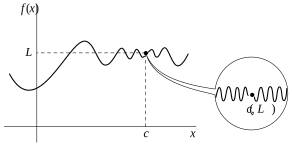
\includegraphics{typicallimit}

(a) \; $\displaystyle \lim_{x \to c} f(x) = L$

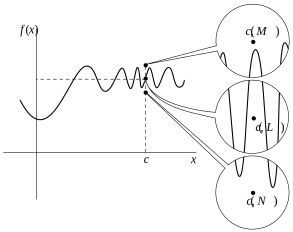
\includegraphics{inexistentlimit}

(b) \; Limite Inexistente
\end{center}
\caption{}\label{fig:exgraphlimits}
\end{figure}

\begin{theorem}\label{teo:slopelimit} A inclinação de $f$ é dada pelo limite
$$
  f'(a) = \lim_{\Dx \to 0} \frac{f(a+\Dx) - f(a)}{\Dx}.
$$
\end{theorem}

Em palavras, a inclinação de $f$ em $a$ é o limite da razão entre a
variação em $f(x)$ e a variação em $x$, tomado à medida que a variação
em $x$ se aproxima de zero. O Teorema~\ref{teo:slopelimit} pode ser
demonstrado apenas pela comparação das definições de limite e inclinação.
A inclinação existe exatamente quando o limite existe; e quando ambos
existem, eles são iguais. Note que a razão
$$
  \frac{f(a+\Dx) - f(a)}{\Dx}
$$
é indefinida quando $\Dx = 0$.

A inclinação de $f$ em $a$ também é igual ao limite
$$
  f'(a) = \lim_{x \to a} \frac{f(x) - f(a)}{x - a}.
$$
Isto pode ser visto se fixarmos
\begin{eqnarray*}
  \Dx & = & x - a, \\
  x & = & a + \Dx.
\end{eqnarray*}
Então, quando $x \approx a$ mas $x \ne a$, temos que $\Dx \approx 0$ mas
$\Dx \ne 0$ e
$$
  \frac{f(x) - f(a)}{x - a} = \frac{f(a + \Dx) - f(a)}{\Dx} \approx f'(a).
$$

Às vezes um limite pode ser avaliado se reconhecermos que ele é uma
derivada e usarmos o Teorema~\ref{teo:slopelimit}.

\begin{example}\label{ex:cap3p3ex1}
  Avalie $\displaystyle \lim_{\Dx \to 0} \frac{(3 + \Dx)^2 - 9}{\Dx}.$

  Seja $F(x) = x^2$. O limire dado é apenas $F'(3)$.
  \begin{eqnarray*}
    F'(3) & = & \lim_{\Dx \to 0} \frac{F(3 + \Dx) - F(3)}{\Dx} =
      \lim_{\Dx \to 0} \frac{(3 + \Dx)^2 - 9}{\Dx}, \\
    F'(3) & = & 2 \cdot 3 = 6.
  \end{eqnarray*}
  Portanto,
  $$
    \lim_{\Dx \to 0} \frac{(3 + \Dx)^2 - 9}{\Dx} = 6.
  $$
\end{example}

O símbolo $x$ em
$$
  \lim_{x \to c} f(x)
$$
é um exemplo de ``variável artificial\tnote{Do inglês: ``dummy variable.''}.''
O valor do limite não depende de $x$ de maneira nenhuma. Entretanto, ele
depende de $c$. Se substituirmos $c$ por uma variável $u$, obtemos uma
nova função
$$
  L(u) = \lim_{x \to u} f(x).
$$

Um limite $\displaystyle \lim_{x \to c} f(x)$ é geralmente calculado da
seguinte maneira:
\begin{stepanalysis}
  \item Considere $x$ infinitamente próximo, mas não igual a $c$, e
        simplifique $f(x)$.
  \item Calcule a parte padronizada $\std(f(x))$.
\end{stepanalysis}
\emph{Conclusão:} Se o limite $\displaystyle \lim_{x \to c} f(x)$ existir,
ele deve ser igual a $\std(f(x))$.

\begin{examplecont}{ex:cap3p3ex1}
  Em vez de usarmos a derivada, podemos calcular diretamente
  $$
    \lim_{\Dx \to 0} \frac{(3 + \Dx)^2 - 9}{\Dx}.
  $$
  \begin{stepanalysis}
    \item Seja $\Dx \approx 0$ mas $\Dx \ne 0$. Então
    $$
      \frac{(3 + \Dx)^2 - 9}{\Dx} = \frac{9 + 6 \Dx + \Dx^2 - 9}{\Dx} =
        \frac{6 \Dx + \Dx^2}{\Dx} = 6 + \Dx.
    $$
    \item Tomando-se a parte padronizada, temos
    $$
      \std \frac{(3 + \Dx)^2 - 9}{\Dx} = \std(6 + \Dx) = 6.
    $$
    Portanto, o limite é igual a $6$. (Veja Figura~\ref{fig:cap3p3ex1}
  \end{stepanalysis}
\end{examplecont}

\includefig[$f(\Dx) = \frac{(3 + \Dx)^2 - 9}{\Dx}$]{cap3p3ex1}

\begin{example}
  Determine $\displaystyle \lim_{t \to 4} (t^2 + 3t - 5)$.

  \begin{stepanalysis}
    \item Seja $t$ infinitamente próximo mas não igual a $4$.
    \item Tomamos a parte padronizada.
    $$
      \std(t^2 + 3t - 5) = 4^2 + 3 \cdot 4 - 5 = 23,
    $$
    logo o limite é $23$.
  \end{stepanalysis}
\end{example}

\begin{example}
  Determine $\displaystyle \lim_{x \to 2} \frac{x^2 + 3x - 10}{x^2 - 4}$.

  \begin{stepanalysis}
    \item Desta vez, o termo dentro do limite é indefinido para $x = 2$.
    Fazendo-se $x \approx 2$, mas $x \ne 2$, temos
    $$
      \frac{x^2 + 3x - 10}{x^2 - 4} = \frac{(x - 2)(x + 5)}{(x - 2)(x + 2)}
        = \frac{x + 5}{x + 2}.
    $$
    \item $\displaystyle \st{\frac{x^2 + 3x - 10}{x^2 - 4}} =
             \st{\frac{x + 5}{x + 2}} = \frac{2 + 5}{2 + 2} = \frac{7}{4}$.\\
    Portanto, \hspace{1.5em}
      $\displaystyle \lim_{x \to 2} \frac{x^2 + 3x - 10}{x^2 - 4} =
        \frac{7}{4}$.
  \end{stepanalysis}
\end{example}

\begin{example}
  Determine $\displaystyle \lim_{x \to 0}
    \left(\frac{(2/x)+3}{(3/x)-1}\right)$.
  \begin{stepanalysis}
  \item Tomando $x \approx 0$ mas $x \ne 0$,
        $$
          \frac{(2/x) + 3}{(3/x) - 1} = \frac{2 + 3x}{3 - x}.
        $$
  \item $\displaystyle \st{\frac{(2/x)+3}{(3/x)-1}} =
          \st{\frac{2 + 3x}{3 - x}} = \frac{2}{3}$.

        Deste modo, o limite existe e é igual a $\frac{2}{3}$.
  \end{stepanalysis}
\end{example}

\begin{example}
  Determine $\displaystyle \lim_{x \to 9} \frac{\sqrt{x} - 3}{x-9}$.
  \begin{stepanalysis}
  \item Tomando $x \approx 9$ mas $x \ne 9$,
        $$
          \frac{\sqrt{x}-3}{x-9} =
            \frac{(\sqrt{x}-3)(\sqrt{x}+3)}{(x-9)(\sqrt{x}+3)} =
            \frac{x - 9}{(x-9)(\sqrt{x}+3} = \frac{1}{\sqrt{x} + 3}.
        $$
  \item $\displaystyle \std{\sqrt{x}-3}{x - 9} = \st{\frac{1}{\sqrt{x}+3}} = \frac{1}{\sqrt{9}+3} = \frac{1}{6}$.

        portanto, o limite existe e é $\frac{1}{6}$.
  \end{stepanalysis}
\end{example}

As regras mostradas no Capítulo~\ref{chp:reals} para o cálculo de partes
padronizadas levam diretamente às regras para os limites. Listamos estas
regras na Tabela~\ref{tab:limitrules}. As regras para limites podem ser
aplicadas sempre que os dois limites $\dslim{x \to c} f(x)$ e
$\dslim{x \to c} g(x)$ existam.

\begin{includetable}{limitrules}
\setlength{\tabcolsep}{0.7em}
  \begin{tabular}{l|l}
  \hline
    \multicolumn{1}{c|}{Regra para Parte Padronizada} &
      \multicolumn{1}{c}{Regra para Limite} \\
  \hline
    $\std(kb) = k \std(b)$, $k$ real &
    $\dslim{x \to c} k f(x) = k \dslim{x \to c} f(x)$ \\
    $\std(a + b) = \std(a) + \std(b)$ &
    $\dslim{x \to c} (f(x) + g(x)) = \dslim{x \to c} f(x) +
      \dslim{x \to c} g(x)$ \\
    $\std(a b) = \std(a) \cdot \std(b)$ &
    $\dslim{x \to c} (f(x) g(x)) = \dslim{x \to c} f(x) \cdot
      \dslim{x \to c} g(x)$ \\
    $\std(a/b) = \std(a) / \std(b)$, se $|\std(b)| > 0$ &
    $\dslim{x \to c} (f(x) / g(x)) = \dslim{x \to c} f(x) /
      \dslim{x \to c} g(x)$, se $\dslim{x \to c} g(x) \ne 0$  \\
    $\std(\sqrt[n]{a}) = \sqrt[n]{\std(a)}$, se $a > 0$ &
    $\dslim{x \to c} \sqrt[n]{f(x)} = \vclear{\sqrt[n]{\lim\limits_{x \to c} f(x)}}$
      se $\dslim{x \to c} f(x) > 0$ \\
  \hline
  \end{tabular}
\end{includetable}

\begin{example}
  Determine $\dslim{x \to 1} (x^2 - 2x)\sqrt{(x^2-1)/(x-1)}$.

  Todos os limites envolvidos existem, logo podemos usar as regras de limites
  para calcular o limite como se segue. Primeiramente, encontramos o limite
  da expressão dentro do radical.
  $$
    \lim_{x \to 1} \frac{x^2 - 1}{x - 1} =
      \lim_{x \to 1} \frac{(x-1)(x+1)}{x-1} = \lim_{x \to 1} (x+1) = 2.
  $$
  Agora, encontramos a resposta para o problema original.
  \begin{eqnarray*}
    \lim_{x \to 1} (x^2 - 2x)\sqrt{(x^2-1)/(x-1)} & = &
      \lim_{x \to 1} (x^2 - 2x) \cdot \sqrt{\lim_{x \to 1} (x^2-1)/(x-1)} \\
    & = & (1 -2) \sqrt{2} = -\sqrt{2}.
  \end{eqnarray*}
\end{example}

Há três maneiras nas quais um limite $\dslim{x \to c} f(x)$ pode não
existir:
\begin{enumerate}[(1)]
\item $f(x)$ é indefinido para algum $x$ infinitamente próximo, mas não igual
      a $c$.
\item $f(x)$ é infinito para algum $x$ infinitamente próximo, mas não igual a
      $c$.
\item A parte padronizada de $f(x)$ é diferente para distintos números $x_1$,
      $x_2$ infinitamente próximos, mas não iguais a $c$.
\end{enumerate}

\begin{example}\label{ex:cap3p3ex7}
$\dslim{x \to 0} \sqrt{x}$ não existe pois $\sqrt{x}$ é indefinido para
qualquer número infinitesimal negativo $x$. (Veja
Figura~\ref{fig:cap3p3exs789}(a).)
\end{example}

\begin{example}\label{ex:cap3p3ex8}
$\dslim{x \to 0} 1/x^2$ não existe pois $1/x^2$ é infinito para qualquer
infinitesimal $x \ne 0$. (Veja Figura~\ref{fig:cap3p3exs789}(b).)
\end{example}

\begin{figure}
\begin{minipage}{0.3\textwidth}
\centering
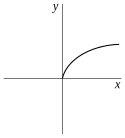
\includegraphics{cap3p3ex7}\\
(a) \; $y = \sqrt{x}$
\end{minipage}%
\hfill%
\begin{minipage}{0.3\textwidth}
\centering
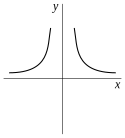
\includegraphics{cap3p3ex8}\\
(b) \; $y = \dfrac{1}{x^2}$
\end{minipage}%
\hfill%
\begin{minipage}{0.3\textwidth}
\centering
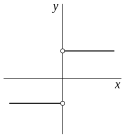
\includegraphics{cap3p3ex9}\\
(c) \; $y = \dfrac{x}{|x|}$
\end{minipage}%
\caption{}\label{fig:cap3p3exs789}
\end{figure}

\begin{example}\label{ex:cap3p3ex9}
$\dslim{x \to 0} x/|x|$ não existe pois 
$$
  \st{\frac{x}{|x|}} = \left\{ \begin{array}{rl}
                          1 & \text{ se } x > 0, \\
                         -1 & \text{ se } x < 0.
                       \end{array} \right.
$$
(Veja Figura~\ref{fig:cap3p3exs789}(b).)
\end{example}

Nos três exemplos anteriores, a função se comporta de maneira diferente de
um dos lados do ponto $0$ com relação ao seu comportamento do outro lado.
Para tais funções, é útil definir o conceito de
\newdef[limite!lateral]{limites laterais}.

Dizemos que
$$
  \lim_{x \to c^+} f(x) = L
$$
se, para todo $x > c$ tal que $x \approx c$, é verdade que $f(x) \approx L$.
Já o limite
$$
  \lim_{x \to c^-} f(x) = L
$$
significa que, para todo $x < c$ tal que $x \approx c$, é verdade que
$f(x) \approx L$. Estes dois tipos de limites, ilustrados na
Figura~\ref{fig:onesidedlimits}, são chamados respectivamente de
\newdef[limite!pela direita]{limite pela direita} e
\newdef[limite!pela esquerda]{limite pela esquerda}.

\begin{includepic}[Limites laterais.]{onesidedlimits}{101.02,55.24}
\put(0,0){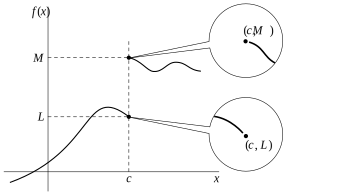
\includegraphics{onesidedlimits}}
\put(80.929,44.409){\normalsize$\lim\limits_{x \to c^{+}} f(x) = M$}
\put(80.929,17.306){\normalsize$\lim\limits_{x \to c^{-}} f(x) = L$}
\end{includepic}

\begin{theorem}
% corrigindo erro no enunciado original do teorema 2 na p. 123
O valor de um limite é $L$, ou seja,
$$
  \lim_{x \to c} f(x) = L, % erro no original: estava f(c)
$$
se, e somente se, ambos os limites laterais existem e são iguais a L,
ou seja,
$$
  \lim_{x \to c^-} f(x) = \lim_{x \to c^+} f(x) = L.
$$
\end{theorem}

\begin{proof}
Se $\lim_{x \to c} f(x) = L$, decorre imediatamente da definição que ambos
os limites laterais são $L$.

Para demonstrar a recíproca, assuma que ambos os limites laterais são
iguais a $L$. Seja $x \approx c$, mas $x \ne c$. Então, ou $x < c$,
ou $x > c$. Se $x < c$, então, como $\lim_{x \to c^-} f(x) = L$, temos
que $f(x) \approx L$. Por outro lado, se $x > c$, então $\lim_{x \to c}
f(x) = L$ nos dá $f(x) \approx L$. Assim, em ambos os casos,
$f(x) \approx L$. Isto nos mostra que $\lim_{x \to c} f(x) = L$.
\end{proof}

Quando um limite não existe, é possível que nenhum dos limites laterais
exista, que apenas um dele exista, ou que ambos os limites laterais existam
mas possuindo valores diferentes.

\begin{examplecont}{ex:cap3p3ex7} \; $\dslim{x \to 0^+} \sqrt{x} = 0$,
  \hspace{1.5em} e \hspace{1.5em} $\dslim{x \to 0^-} \sqrt{x}$ \; não existe.
\end{examplecont}

\begin{examplecont}{ex:cap3p3ex8} \; Nem \; $\dslim{x \to 0^+} 1/x^2$,
  \hspace{1.5em} nem \hspace{1.5em} $\dslim{x \to 0^-} 1/x^2$ \; existem.
\end{examplecont}

\begin{examplecont}{ex:cap3p3ex9} \; $\dslim{x \to 0^+} x/|x| = 1$,
  \hspace{1.5em} e \hspace{1.5em} $\dslim{x \to 0^-} x/|x| = -1$.
\end{examplecont}

\begin{sectionproblems}
Em cada um dos problemas abaixo, determine se o limite existe ou não.
Nos casos em que o limite existe, calcule o seu valor. Com uma calculadora,
calcule alguns valores da função à medida que a variável se aproxima do 
valor indicado e verifique o que acontece.

\twoexer{$\dslim{t \to 4} 3t^2 + t + 1$}%
        {$\dslim{\Dx \to -1} \dfrac{\Dx^2 + 2\Dx + 1}{\Dx + 1}$}

\twoexer{$\dslim{x \to c} \sqrt{c - x}$}%
        {$\dslim{y \to 0} \dfrac{1}{y^5}$}

\twoexer{$\dslim{x \to 2} \dfrac{x}{x^2 - 4}$}%
        {$\dslim{x \to 2} \dfrac{x^2 - 4}{x - 2}$}

\twoexer{$\dslim{v \to 8} \dfrac{\sqrt{8} - \sqrt{v}}{v - 8}$}%
        {$\dslim{x \to 0} \dfrac{\sqrt{x + 1} - 1}{x}$}

\twoexer{$\dslim{u \to 1} \dfrac{\sqrt[3]{u} - 1}{u - 1}$}%
        {$\dslim{t \to 0} \dfrac{t^3-2t^2+4}{3t^2-5t+7}$}

\twoexer{$\dslim{y \to 0} (\sqrt{1 + 1/y} - \sqrt{1/y})$}%
        {$\dslim{x \to 0} \dfrac{(a + x)^2 - a^2}{x}$}

\twoexer{$\dslim{y \to -1} \dfrac{y^2 + 1}{y + 1}$}%
        {$\dslim{x \to 1} \dfrac{|x-1|}{x-1}$}

\twoexer{$\dslim{x \to 1^+} \dfrac{|x-1|}{x-1}$}%
        {$\dslim{x \to c^-} \sqrt{c-x}$}

\twoexer{$\dslim{z \to 1} \sqrt{z+\sqrt{z+\sqrt{z}}}$}%
        {$\dslim{x \to a} \sqrt{|a-x|}$}

\twoexer{$\dslim{x \to 0^+} x \sqrt{1 + x^{-2}}$}%
        {$\dslim{x \to 0^-} x \sqrt{1 + x^{-2}}$}

\twoexer{$\dslim{t \to 0} \dfrac{1 + 2t^{-1}}{3 - 4t^{-1}}$}%
        {$\dslim{x \to 0} \dfrac{3 + 4x^{-1} - 5x^{-2}}{6-x^{-1}+3x^{-2}}$}

\twoexer{$\dslim{\Dx \to 0} \dfrac{(x + \Dx)^2 - x^2}{\Dx}$}%
        {$\dslim{\Dx \to 0} \dfrac{\dfrac{1}{x + \Dx}-\dfrac{1}{x}}{\Dx}$ \;
         ($x \ne 0$)}

\twoexer{$\dslim{\Dt \to 0} \dfrac{\sqrt{t + \Dt}-\sqrt{t}}{\Dt}$ \; ($t > 0$)}%
        {$\dslim{\Dt \to 0} \dfrac{(t + \Dt)^{1/5} - t^{1/5}}{\Dt}$ \; ($t > 0$)}

\twoexer{$\dslim{\Dx \to 0} \dfrac{(x - \Dx)^3 - x^3}{\Dx}$}%
        {$\dslim{\Dx \to 0} \dfrac{\dfrac{x + \Dx}{x + \Dx + 1}-\dfrac{x}{x+1}}{\Dx}$ \; ($x~\ne~-1$)}

\twoexer{$\dslim{\Dx \to 0^-} \dfrac{|(1+\Dx)^3-(1+\Dx)|}{\Dx}$}%
        {$\dslim{\Dx \to 0^+} \dfrac{|(1+\Dx)^3-(1+\Dx)|}{\Dx}$}

\exer{$\dslim{\Dx \to 0^-} \dfrac{\sqrt{1 - (1+\Dx)^2}}{\Dx}$}

\end{sectionproblems}

\section{Continuidade}
\label{sec:continuity}

Intuitivamente, uma curva $y = f(x)$ é contínua se ela forma um gráfico
sem quebras, isto é, toda vez que $x_1$ estiver próximo de $x_2$, teremos
que $f(x_1)$ estará próximo de $f(x_2)$. Para transformarmos esta ideia
intuitiva em uma definição matemática, substituiremos ``próximo'' por
``infinitamente próximo.''

% TODO: definir environment definition*
\begin{definition*}
Dizemos que uma função $f$ é \index{continuidade}
\newdef[função!contínua em um ponto]{contínua} em um ponto $c$ se:
\begin{enumerate}[(i)]
\item $f$ está definida em $c$;
\item para todo $x$ infinitamente próximo de $c$, temos que $f(x)$ está
      infinitamente próximo de $f(c)$.
\end{enumerate}
\end{definition*}

Se $f$ não é contínua em $c$, dizemos que ela é \newdef[função!descontínua em um ponto]{descontínua} em $c$.

Quando $f$ é contínua em $c$, a parte inteira da curva onde $x \approx c$
será visível em um microscópio infinitesimal centrado em $(c, f(c))$,
conforme mostrado na Figura~\ref{fig:continuitygraph}(a). Mas se $f$ é
descontínua em $c$, alguns valores de $f(x)$ onde $x \approx c$ ou estarão
indefinidos, ou estarão fora do campo de visão do microscópio, conforme
Figura~\ref{fig:continuitygraph}(b).

Continuidade, como a derivada, pode ser expressada em termos de limites.
Novamente, a prova decorre imediatamente das definições.

\begin{figure}
\begin{center}
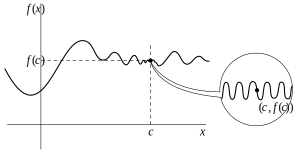
\includegraphics{continuitygraph-a}

(a) $f$ contínua em $c$.

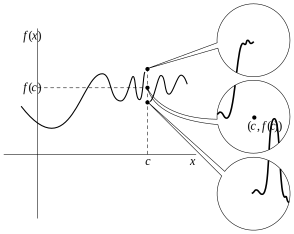
\includegraphics{continuitygraph-b}

(b) $f$ descontínua em $c$.
\end{center}
\caption{}\label{fig:continuitygraph}
\end{figure}

\begin{theorem}
A função $f$ é contínua em $c$ se, e somente se,
$$
  \lim_{x \to c} f(x) = f(c).
$$
\end{theorem}

Como aplicação, temos um conjunto de regras para combinar funções contínuas.
Elas podem ser demonstradas tanto pelas regras correspondentes para limites
(Tabela~\ref{tab:limitrules} na Seção~\ref{sec:limits}) ou pelo cálculo de
partes padronizadas.

\begin{theorem}\label{teo:continuityrules}
Suponha que $f$ e $g$ sejam contínuas em $c$.
\begin{enumerate}[(i)]
\item Para qualquer constante $k$, a função $k \cdot f(x)$ é contínua em $c$.
\item $f(x) + g(x)$ é contínua em $c$.
\item $f(x) \cdot g(x)$ é contínua em $c$.
\item Se $g(c) \ne 0$, então $f(x)/g(x)$ é contínua em $c$.
\item Se $f(c)$ é positivo e $n$ é um inteiro, então $\sqrt[n]{f(x)}$ é
      contínua em $c$.
\end{enumerate}
\end{theorem}

Através da aplicação repetida do Teorema~\ref{teo:continuityrules}, vemos
que todas as funções a seguir são contínuas em $c$.
\begin{itemize}
\item Funções polinomiais.
\item Funções racionais $f(x)/g(x)$, onde $f(x)$ e $g(x)$ são polinômios e
      $g(c) \ne 0$.
\item Funções do tipo $f(x) = x^r$, com $r$ racional e $x > 0$.
\end{itemize}

Às vezes, uma função $f(x)$ é indefinida em um ponto $x = c$, enquanto que
o limite
$$
  L = \lim_{x \to c} f(x)
$$
existe. Quando isto acontece, podemos fazer a função contínua em $c$
definindo $f(c) = L$.

\begin{example}
Seja $f(x) = \dfrac{x^2 + x - 2}{x - 1}$.

Em qualquer ponto $c \ne 1$, $f$ é contínua. Mas $f(1)$ é indefinido, logo
$f$ é descontínua em $1$. Entretanto,
$$
  \lim_{x \to 1} \frac{x^2 + x - 2}{x - 1} =
    \lim_{x \to 1} \frac{(x - 1)(x + 2)}{x - 1} = 3.
$$
Podemos fazer $f$ contínua em $1$ definindo
$$
  f(x) = \left\{ \begin{array}{cl}
           \dfrac{x^2 + x - 2}{x - 1} & \text{ se } x \ne 1, \\[2ex]
           3 & \text{ se } x = 1.
         \end{array} \right.
$$
(Veja Figura~\ref{fig:cap3p4ex1}.)
\end{example}

\begin{figure}
\begingroup
\begin{center}
\setlength{\unitlength}{1mm}
\begin{picture}(62.81,46.39)
\put(0,0){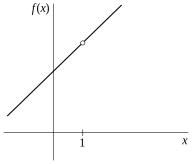
\includegraphics{cap3p4ex1a}}
\put(24.826,31.219){\normalsize$f(1)$ indefinido}
\put(22.815,21.236){\normalsize$f(x) = \dfrac{x^2 + x - 2}{x - 1}$}
\end{picture}
%
\begin{picture}(62.81,46.39)
\put(0,0){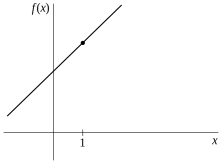
\includegraphics{cap3p4ex1b}}
\put(26.014,32.883){\normalsize$f(1) = 3$}
\put(24.005,20.336){\normalsize$f(x) =
         \left\{ \begin{array}{cl}
           \frac{x^2 + x - 2}{x - 1} & \text{ se } x \ne 1, \\[2ex]
           3 & \text{ se } x = 1.
         \end{array} \right.$}
\end{picture}
\end{center}
\endgroup
\caption{}\label{fig:cap3p4ex1}
\end{figure}

Em termos de uma variável dependente $y = f(x)$, a definição de continuidade
assume a seguinte forma, onde $\Dy = f(c + \Dx) - f(c)$.

\begin{quote}
Dizemos que $y$ é contínua em $x = c$ se:
\begin{enumerate}[(i)]
\item $y$ está definida em $x = c$.
\item Sempre que $\Dx$ é um infintésimo, temos que $\Dy$ é um infinitésimo.
\end{enumerate}
\end{quote}

Resumindo, dada uma função $y = f(x)$ definida em $x = c$, todas as
afirmações abaixo são equivalentes:
\begin{enumerate}[(1)]
\item $f$ é contínua em $c$.
\item Sempre que $x \approx c$, temos que $f(x) \approx f(c)$.
\item Sempre que $\std(x) = c$, temos que $\std(f(x)) = f(c)$.
\item $\lim_{x \to c} f(x) = f(c)$.
\item $y$ é contínua em $x = c$.
\item Sempre que $\Dx$ é um infinitésimo, temos que $\Dy$ é um
      infinitésimo.
\end{enumerate}

Nosso próximo teorema nos diz que diferenciabilidade implica continuidade.
Ou seja, o conjunto de funções diferenciáveis em $c$ é um subconjunto das
funções contínuas em $c$. (Veja Figura~\ref{fig:realfuncclasses}.)

\includefig{realfuncclasses}

\begin{theorem}\label{teo:diffimpliescont}
Se $f$ é diferenciável em $c$, então $f$ é contínua em $c$.
\end{theorem}

\begin{proof}
Seja $y = f(x)$ e seja $\Dx$ um infinitésimo não nulo. Então, $\Dy/\Dx$ está
infinitamente próximo de $f'(c)$, logo é um número finito. Portanto,
$\Dy = \Dx(\Dy/\Dx)$ é o produto entre um infinitésimo e um número finito,
logo $\Dy$ é um infinitésimo.
\end{proof}

Por exemplo, as funções transcendentais $\sen x$, $\cos x$, $\e^x$ são
contínuas para todo $x$, e $\ln x$ é contínua para $x > 0$.
O Teorema~\ref{teo:diffimpliescont} pode ser usado para demonstrar que
combinações entre estas funções são contínuas.

\begin{example}
  Encontre o maior domínio possível para o qual a função
  $$
    f(x) = \frac{\sen x \ln(x + 1)}{x^2 - 4}
  $$
  é contínua.

  A função $\sen x$ é contínua para todo $x$, enquanto que $\ln(x + 1)$ é
  contínua sempre que $x + 1 > 0$, ou seja, $x > -1$. Portanto, o numerador
  $\sen x \ln(x + 1)$ é contínuo sempre que $x > -1$. O denominador $x^2-4$
  é contínuo para todo $x$ mas é zero quando $x = \pm 2$. Deste modo, $f(x)$
  é contínua sempre que $x > -1$ e $x \ne 2$.
\end{example}

Os próximos dois exemplos apresentam funções que são contínuas mas \emph{não}
diferenciáveis em um ponto $c$.

\begin{example}
  A função $y = x^{1/3}$ é contínua mas não diferenciável em $x = 0$.
  (Veja Figura~\ref{fig:nondifffunc}(a).). Vimos, anteriormente, que esta
  função não é diferenciável em $x = 0$. Ela é contínua em $0$ pois, se
  $\Dx$ é um infinitésimo, então o $\Dy$ também é, onde
  $$
    \Dy = (0 + \Dx)^{1/3} - 0^{1/3} = (\Dx)^{1/3}.
  $$
\end{example}

\begin{example}
  A função valor absoluto $y = |x|$ é contínua mas não diferenciável no
  ponto $x = 0$. (Veja Figura~\ref{fig:nondifffunc}(b).)

  Já demonstramos que a sua derivada não existe em $x = 0$. Para verificar
  que a função é contínua em $0$, note que para qualquer infinitésimo $\Dx$,
  $$
    \Dy = |0 + \Dx| - |0| = |\Dx|,
  $$
  logo $\Dy$ é um infinitésimo.
\end{example}

\begin{figure}
\begin{minipage}{60.91mm}
\centering
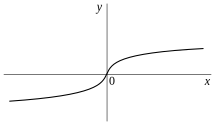
\includegraphics{nondifffunc-a}

(a) $y = x^{1/3}$
\end{minipage}
\hfill
\begin{minipage}{43.58mm}
\centering
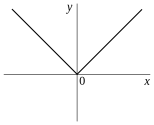
\includegraphics{nondifffunc-b}

(b) $y = |x|$
\end{minipage}
\caption{}\label{fig:nondifffunc}
\end{figure}

A trajetória de uma bola que está quicando é uma série de parábolas,
conforme Figura~\ref{fig:bouncingball}. A curva é contínua em todos
os pontos. Nos pontos $a_1$, $a_2$, $a_3$, \ldots onde a bola quica,
a curva é contínua mas não diferenciável. Em todos os outros pontos,
a curva é contínua e diferenciável.

\begin{includepic}[Trajetória de uma bola que quica.]{bouncingball}{104.14,35.64}
\normalsize
\put(0,0){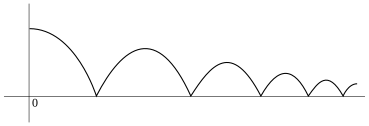
\includegraphics{bouncingball}}
\put(27.1196816257409, 5.49025317527519){\hspace{-0.5em}$a_1$}
\put(53.94029353655094,5.49025317527519){\hspace{-0.5em}$a_2$}
\put(73.73377081569291, 5.49025317527519){\hspace{-0.5em}$a_3$}
\put(87.20056731583404, 5.49025317527519){\hspace{-0.5em}$a_4$}
\put(96.87135196161444, 5.49025317527519){\hspace{-0.5em}$a_5$}
\end{includepic}

Na teoria cinética dos gases clássica, assumimos que uma molécula de gás
se desloca a velocidade constante em linha reta, exceto no instante de
tempo em que ela colide com outra molécula ou com a parede do recipiente
que contém o gás. Sua trajetória descreve um zigue-zague no espaço, conforme
a Figura~\ref{fig:brownianmotion}.

\includefig[Movimento de uma molécula em um gás ideal.]{brownianmotion}

A posição no espaço tridimensional no instante $t$ pode ser representada
por três funções
$$
  x = f(t), \hspace{1.5em} y = g(t), \hspace{1.5em} z = h(t).
$$
Todas as três funções, $f$, $g$ e $h$ são contínuas para todos os valores
de $t$. No instante $t$ de uma colisão, ao menos uma, e geralmente todas as
três derivadas $\dx/\dt$, $\dy/\dt$, $\dz/\dt$ serão indefinidas pois a
velocidade ou a direção da molécula muda subitamente. Em qualquer outro
instante $t$, quando nenhuma colisão está acontecendo, todas as três
derivadas $\dx/\dt$, $\dy/\dt$, $\dz/\dt$ existirão.

As funções que encontraremos comumente neste livro serão definidas e
possuirão derivada em todos os pontos, à exceção possível de um conjunto
finito de pontos em um intervalo. O gráfico de tal função será uma curva
suave onde a derivada existe. Nos pontos onde a curva possuir um bico afiado
(como no ponto $x = 0$ para a função $y = |x|$) ou uma tangente vertical
(como no ponto $x = 0$ para a função $y = x^{1/3}$), a função é contínua mas
não diferenciável (veja Figura~\ref{fig:excontbutnotdiff}). Nos pontos onde
a função é indefinida ou dá um salto, ou o valor se aproxima de infinito,
ou oscila violentamente, a função é descontínua (veja
Figura~\ref{fig:exfuncdiscontinuous}).

\includefig[Pontos onde $f$ é contínua mas não diferenciável.]{excontbutnotdiff}

\includefig[Pontos onde $f$ é descontínua.]{exfuncdiscontinuous}

O próximo teorema é similar à Regra da Cadeia para derivadas.

\begin{theorem}
  Se $f$ é contínua em $c$ e $G$ é contínua em $f(c)$, então a função
  $$
    g(x) = G(f(x))
  $$
  também é contínua em $c$. Ou seja, a composição de duas funções contínuas
  é uma função contínua
\end{theorem}

\begin{proof}
  Seja $x$ infinitamente próximo, mas não igual a $c$. Então
  $$
    \std(g(x)) = \std(G(f(x))) = G(\std(f(x))) = G(f(c)) = g(c).
  $$
\end{proof}

Por exemplo, as funções a seguir são contínuas:
$$
  \begin{array}{rcl@{\hspace{1em}}l}
    f(x) & = & \sqrt{x^2 + 1}, & \text{ para todo } x, \\
    g(x) & = & |x^3 - x|, & \text{ para todo } x, \\
    h(x) & = & (1 + \sqrt{x})^{1/3}, & \text{ para } x > 0, \\
    j(x) & = & \e^{\sen x}, & \text{ para todo } x, \\
    k(x) & = & \ln|x|, & \text{ para } x \ne 0.
  \end{array}
$$
A seguir, apresentamos dois exemplos que ilustram dois tipos de
descontinuidades.

\begin{example}
  A função
  $$
    g(x) = \frac{x^2 - 3x + 4}{4(x-1)(x-2)}
  $$
  é contínua para todo número real exceto $x = 1$ e $x = 2$. Nestes dois
  pontos, $g(x)$ é indefinido (Figura~\ref{fig:cap3p4ex5}).
\end{example}

\includefig[\normalsize$y = \frac{x^2 - 3x + 4}{4(x-1)(x-2)}$]{cap3p4ex5}

\includefig[\normalsize$y = \floor{x}$]{cap3p4ex6}

\begin{example}\label{ex:floorfunc}
  A \newdef[função!maior inteiro]{função maior inteiro}%
  \tnote{Também denominada \emph{função piso}.\index{função!piso}}, denotada por
  $\floor{x}$, cujo gráfico é ilustrado na Figura~\ref{fig:cap3p4ex6},
  é definida por
  $$
    \floor{x} = \text{maior inteiro } n \text{ tal que } n \le x.
  $$
  Assim, $\floor{x} = 0$ se $0 \le x < 1$, $\floor{x} = 1$,
  se $1 \le x < 2$, $\floor{x} = 2$ se $2 \le x < 3$, e daí em diante.
  Para $x$ negativo, temos $\floor{x} = -1$ se $-1 \le x < 0$,
  $\floor{x} = -2$ se $-2 \le x < -1$, e daí em diante. Por exemplo,
  $$
    \floor{7,362} = 7, \hspace{1.5em}
    \floor{\pi} = 3, \hspace{1.5em}
    \floor{-2,43} = -3.
  $$
  Para todo inteiro $n$, $\floor{n}$ é igual a $n$. A função $\floor{x}$
  é contínua quando $x$ não é um inteiro, mas é descontínua quando $x$ é
  um inteiro $n$. Em um inteiro $n$, os limites laterais existem, mas são
  diferentes:
  $$
    \lim_{x \to n^-} f(x) = n-1, \hspace{1.5em}
    \lim_{x \to n^+} f(x) = n.
  $$
  O gráfico de $\floor{x}$ se parece com uma escada. Ele tem um degrau,
  ou salto descontínuo, para cada inteiro $n$. A função $\floor{x}$ será
  útil na última seção deste capítulo. Algumas calculadoras têm uma tecla
  para a função maior inteiro, ou para a função similar que dá $\floor{x}$
  para $x$ positivo e $\floor{x} + 1$ para $x$ negativo.
\end{example}

Funções que são ``contínuas em um intervalo'' desempenharão um papel
importante neste capítulo. Os intervalos foram discutidos na
Seção~\ref{sec:realline}. Recorde que os intervalos fechados têm a forma
$$
  [a, b],
$$
enquanto que os intervalos abertos têm uma das formas
$$
  (a, b), \hspace{1.5em} (a, \infty), \hspace{1.5em}, (-\infty, b),
  \hspace{1.5em} (-\infty, \infty),
$$
e intervalos semi-abertos têm uma das formas
$$
  [a, b), \hspace{1.5em} (a, b], \hspace{1.5em} [a, \infty),
  \hspace{1.5em} (-\infty, b].
$$
Nestes intervalos, $a$ é chamado de \newdef{extremo inferior} e $b$ de
\newdef{extremo superior}. O símbolo $-\infty$ indica que não há extremo
inferior, enquanto que $\infty$ indica que não há extremo superior.

\begin{definition*}
  Dizemos que $f$ é \index{continuidade!em intervalo aberto}
\newdef[função!contínua!em intervalo aberto]{contínua em um intervalo
aberto $I$} se $f$ é contínua em todo ponto $c$ de $I$. Se, além disso, ela
for diferenciável em todo ponto de $I$, então dizemos que $f$ é
\index{diferenciabilidade!em intervalo aberto}
\newdef[função!diferenciável em intervalo aberto]{diferenciável em $I$}.
\end{definition*}

Para definirmos o significado de uma função contínua em um intervalo fechado,
introduzimos as noções de continuidade pela direita e continuidade pela
esquerda por meio de limites laterais.

\begin{definition*}
  Dizemos que $f$ é \index{continuidade!pela direita}
\newdef[função!contínua!pela direita]{contínua pela direita} em $x$ se
$\lim\limits_{x \to c^+} f(x) = f(c)$.

  Dizemos que $f$ é \index{continuidade!pela esquerda}
\newdef[função!contínua!pela esquerda]{contínua pela esquerda} em $x$ se
$\lim\limits_{x \to c^-} f(x) = f(c)$.
\end{definition*}

\begin{examplecont}{ex:floorfunc}
  A função maior inteiro $f(x) = \floor{x}$ é contínua pela direita mas não
  pela esquerda em cada inteiro $n$ pois
  $$
    \floor{n} = n, \hspace{1.5em} \lim_{x \to n^+} \floor{x} = n,
    \hspace{1.5em} \lim_{x \to n^-} \floor{x} = n - 1.
  $$
\end{examplecont}

É fácil verificar que $f$ é contínua em $c$ se, e somente se, $f$ é contínua
tanto pela esquerda quanto pela direita em $c$.

\begin{definition*}
  Dizemos que $f$ é \index{continuidade!em intervalo fechado}
\newdef[função!contínua!em intervalo fechado]{contínua em um intervalo
fechado $[a, b]$} se $f$ é contínua em todo ponto $c$ tal que $a < c < b$,
contínua pela direita em $a$ e contínua pela esquerda em $b$.
\end{definition*}

A Figura~\ref{fig:fcontclosedinter} mostra uma função $f$ contínua em
$[a, b]$.

\includefig[Função $f$ contínua no intervalo ${[}a, b{]}$.]{fcontclosedinter}

\begin{example}
  O semicírculo
  $$
    y = \sqrt{1 - x^2},
  $$
  mostrado na Figura~\ref{fig:fsemicircle}, é contínuo no intervalo fechado
  $[-1, 1]$. Ele é diferenciável no intervalo aberto $(-1, 1)$. Para
  verificar que ele é contínuo pela direita em $x = -1$, seja $\Delta x$
  um infinitésimo positivo. Então,
  \begin{eqnarray*}
    y & = & \sqrt{1 - (-1)^2} = 0 \\
    y + \Dy & = & \sqrt{1 - (-1 + \Dx)^2} = \sqrt{1 - (1 - 2\Dx + \Dx^2)} \\
    & = & \sqrt{2 \Dx - \Dx^2} = \sqrt{(2 - \Dx)\Dx}.
  \end{eqnarray*}
  Portanto
  $$
    \Dy = \sqrt{(2-\Dx)\Dx}.
  $$
  O número dentro do radical é um infinitésimo positivo, logo $\Dy$ é um
  infinitésimo. Isto mostra que a função é contínua pela direita em
  $x = -1$. Um argumento similar mostra que a função é contínua pela
  esquerda em $x = 1$.
\end{example}

\includefig[$y = \sqrt{1 - x^2}$]{fsemicircle}

\begin{sectionproblems}

Nos Problemas~\ref{prob:chp3p4p1}--\ref{prob:chp3p4p17}, determine o
conjunto de todos os pontos para os quais a função é contínua.

\twoexer{$f(x) = 3x^2 + 5x + 4$\label{prob:chp3p4p1}}%
        {$f(x) = \dfrac{5x + 2}{x^2 + 1}$}

\twoexer{$f(x) = \sqrt{x + 2}$}%
        {$f(x) = \dfrac{x}{x+2}$}

\twoexer{$f(x) = \sqrt{|x - 2| + 1}$}%
        {$f(x) = \dfrac{x + 3}{|x + 3|}$}

\twoexer{$f(x) = \dfrac{x}{x^2 + x}$}%
        {$f(x) = \dfrac{x + 2}{(x-1)(x-3)^{1/3}}$}

\twoexer{$f(x) = \sqrt{4 - x^2}$}%
        {$f(x) = \sqrt{x^2 - 4}$}

\twoexer{$f(x) = \dfrac{1}{x-(1/(x+1))}$}%
        {$g(x) = \dfrac{1}{x} + \dfrac{1}{x-1}$}

\twoexer{$g(x) = \dfrac{x-2}{x-3} + \dfrac{x-3}{x-2}$}%
        {$g(x) = \sqrt{x^3-x}$}

\twoexer{$g(x) = \sqrt[4]{x^2 - x^3}$}%
        {$f(t) = \sqrt{t^{-2} - 1}$}

\exer{$f(t) = \sqrt{t^{-1} - 1}$\label{prob:chp3p4p17}}

\exer{Mostre que $f(x) = \sqrt{x}$ é contínua pela direita em $x = 0$.}

\exer{Mostre que $f(x) = \sqrt{1-x}$ é contínua pela esquerda em $x = 1$.}

\exer{Mostre que $f(x) = \sqrt{1-|x|}$ é contínua no intervalo fechado $[-1, 1]$.}

\exer{Mostre que $f(x) = \sqrt{x} + \sqrt{2-x}$ é contínua no intervalo fechado $[0, 2]$.}

\exer{Mostre que $f(x) = \sqrt{9-x^2}$ é contínua no intervalo fechado $[-3, 3]$.}

\exer{Mostre que $f(x) = \sqrt{x^2-9}$ é contínua nos intervalos $(-\infty, -3]$ e $[3, +\infty)$.}

\hardex{Suponha que a função $f(x)$ é contínua no intervalo fechado
$[a, b]$. Mostre que existe uma função $g(x)$ que é contínua em toda a reta
real e tem valor $g(x) = f(x)$ para $x$ em $[a, b]$.}

\hardex{Suponha que $\lim_{x \to c} f(x) = L$. Prove que a função $g(x)$,
definida por $g(x) = f(x)$ para $x \ne c$ e $g(x) = L$ para $x = c$, é
contínua em $c$.}

\exer{Na curva $y = f(x)$, ilustrada na Figura~\ref{fig:chp3p4p26},
identifique os pontos $x = c$ onde cada uma das condições abaixo ocorre:
\begin{enumerate}[(a)]
\item $f$ é descontínua em $x = c$
\item $f$ é contínua mas não diferenciável em $x = c$.
\end{enumerate}}

\includefig{chp3p4p26}

\end{sectionproblems}

\section{Máximos e Mínimos}
\label{sec:maxmin}

Assumiremos, nesta seção, que $f$ é uma função real cujo domínio é um intervalo
$I$ e que $f$ é contínua em $I$. Um problema que comumente aparece é o de se
encontrar o ponto $c$ onde $f(c)$ assume o seu maior valor, ou o ponto $c$
onde $f(c)$ tem seu menor valor. A derivada mostra a sua utilidade neste
problema. Começamos por definir os conceitos de máximo e mínimo.

\begin{definition*}
  Seja $c$ um número real no domínio $I$ de $f$.
  \begin{enumerate}[(i)]
  \item $f$ tem um \newdef{máximo} em $c$ se $f(c) \ge f(x)$ para todo
        e qualquer número real $x$ em $I$. Neste caso, $f(c)$ é chamado
        o \newdef{valor máximo} de $f$.
  \item $f$ tem um \newdef{mínimo} em $c$ se $f(c) \le f(x)$ para todo
        e qualquer número real $x$ em $I$. Neste caso, $f(c)$ é chamado
        o \newdef{valor mínimo} de $f$.
  \end{enumerate}
\end{definition*}

Quando observamos o gráfico de uma função $f$ contínua em $I$, o máximo
aparecerá como o maior pico e o mínimo como o vale mais baixo
(Figura~\ref{fig:maxmin}).

\includefig[Máximo e mínimo.]{maxmin}

Em geral, todas as possibilidades a seguir podem ocorrer:
\begin{itemize}
\item $f$ não tem máximo em seu domínio $I$.
\item $f$ tem um máximo em exatamente um ponto em $I$.
\item $f$ tem máximos em vários pontos diferentes em $I$.
\end{itemize}

Entretanto, mesmo que $f$ tenha máximos em vários pontos diferentes, $f$ só
pode ter um único valor máximo (se tiver algum). Como $f$ tem um máximo em
$c_1$ e também em $c_2$, então $f(c_1) \ge f(c_2)$ e $f(c_2) \ge f(c_1)$,
portanto $f(c_1)$ e $f(c_2)$ são iguais.

\begin{example}
  Cada uma das funções a seguir, cujos gráficos estão na
  Figura~\ref{fig:nomaxmin}, não possuem máximo nem mínimo:
  \begin{enumerate}[(a)]
  \item $f(x) = 1/x$, \hspace{1.5em} $0 < x$.
  \item $f(x) = x^2$, \hspace{1.5em} $0 < x < 1$.
  \item $f(x) = 2x + 3$.
  \end{enumerate}
\end{example}

\begin{figure}
\begin{minipage}{38.67mm}
\begin{center}
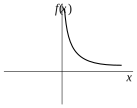
\includegraphics{nomaxmin-a}

(a) $f(x) = \frac{1}{x}, \; 0 < x$
\end{center}
\end{minipage}%
\begin{minipage}{38.67mm}
\begin{center}
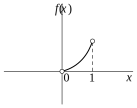
\includegraphics{nomaxmin-b}

(b) $f(x) = x^2, \; 0 < x < 1$
\end{center}
\end{minipage}%
\begin{minipage}{38.67mm}
\begin{center}
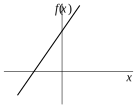
\includegraphics{nomaxmin-c}

(c) $f(x) = 2x + 3$
\end{center}
\end{minipage}
\caption{Sem máximo nem mínimo.}
\label{fig:nomaxmin}
\end{figure}

\section{Máximos e Mínimos -- Aplicações}
\label{sec:maxminappl}

\section{Derivadas e Esboços de Curvas}
\label{sec:derivsketch}

\section{Propriedades de Funções Contínuas}
\label{sec:propcont}

\begin{chapterproblems}
\end{chapterproblems}
